\chapter{Applications}
\label{chap:fw-app}
\index{Application}

%%%%%%%%%%%%%%%%%%%%%%%%%%%%%%%%%%%%%%%%%%%%%%%%%%%%%%%%%%%%%%%%%%%%%%%%%%%%%%%%
In this chapter, we will explain how to make use of the framework
instance created in \autoref{chap:fw-inst} to build a person
re-identification application to realize our main goal of tracking the same person 
across multiple cameras. Besides the main ReID application, we will also 
introduce other applications: skeleton tracking, camera calibration, image 
alignment and green screen image, which are all built on top of our OpenISS 
framework instance.
With the applications added, the architecture of our current system can be 
shown by \autoref{fig:fw-app}.

\begin{figure}
    \centering
    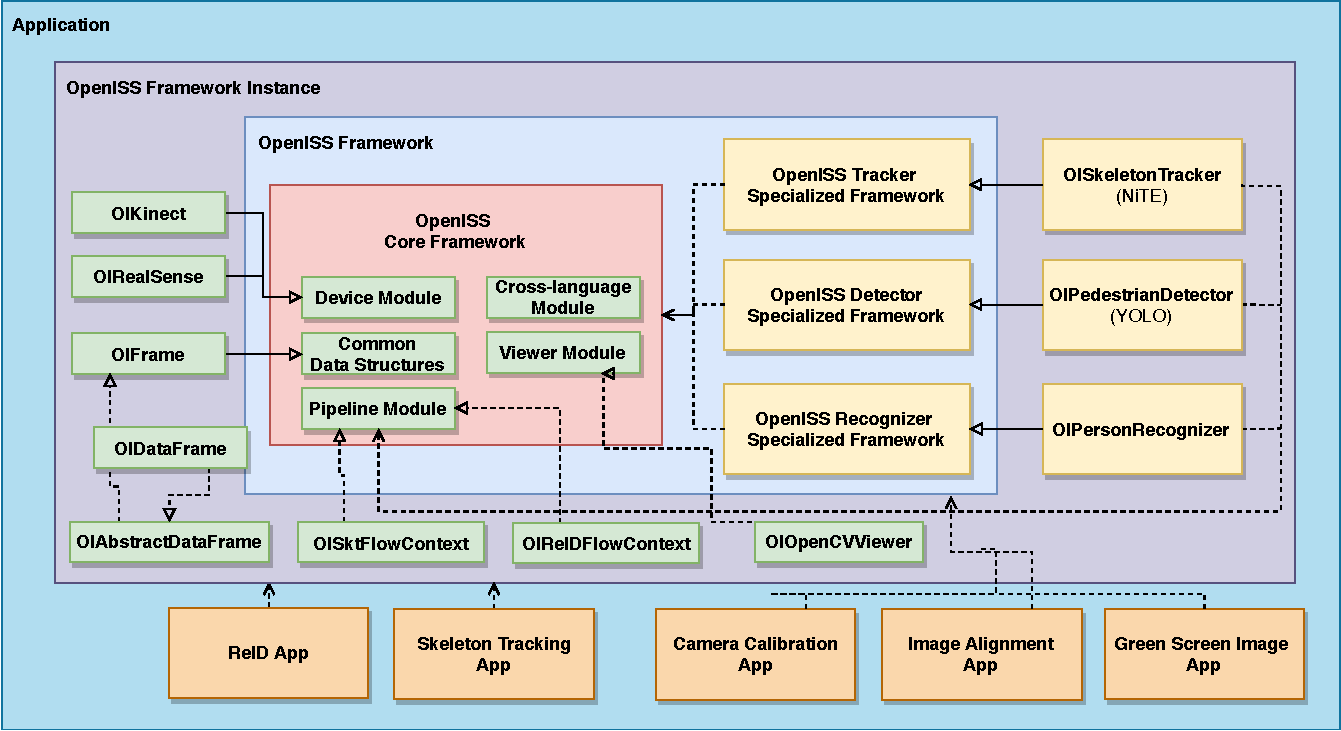
\includegraphics[width=\linewidth]{figures/framework_app.pdf}
    \caption{Applications built on top of our framework instance.}
    \label{fig:fw-app}
\end{figure}

\section{ReID Application}
\label{sec:fw-app-reid}

%In \autoref{sec:fw-design-spec-detector} and
%\autoref{sec:fw-design-spec-recognizer}, we stated our design of both detector
%and recognizer frozen spots.
%In \autoref{sec:fw-inst-detector} and \autoref{sec:fw-inst-recoginzer}, we
%described how we create hot spots for the detector and recognizer frozen spots
%adapting to the specific person detection and person retrieval tasks.
%The combination of them can address the person ReID task which is the main 
%goal 
%of this thesis.
%Also, they all agree with the \texttt{OIFlowable}
%interface to support the pipeline mechanism defined in the core framework.
%In this section, we are going to explain, how we use the framework instance
%described in \autoref{chap:fw-inst} for person re-identification task by
%chaining the proposed hot spots together.

Until now, what we described in the previous chapters is the design and 
implementation of the framework itself. But it cannot solve our
concrete ReID problem directly, since they are just pieces of solution for each 
subproblems. If we would like to use it for a specific task, we need a way to 
organize these fragments so that they can operate following our expectations.
Our ReID application is the software we built using our framework instance to 
address the ReID task which includes person detection and person recognition.

\begin{figure}
    \centering
    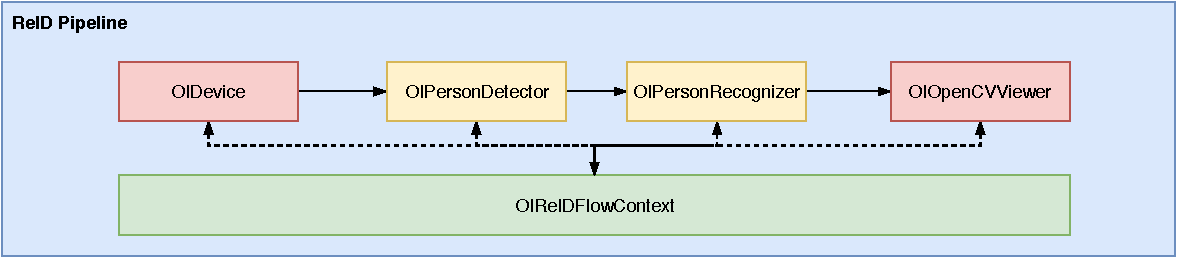
\includegraphics[width=\linewidth]{figures/framework_app_reid_pipeline.pdf}
    \caption[Person re-identification pipeline]
    {Person re-identification pipeline,  the solid line arrow represents
    the pipeline execution order and the dash line arrow represents the
    data flow.}
    \label{fig:fw-app-reid-pipeline}
\end{figure}

As mentioned in \autoref{sec:intro-pbstat}, the person ReID task can be divided
into two portions: one is person detection and the other is person retrieval. 
We have already shown how to create two specialized frameworks for each of these 
two parts. Intuitively, what we
need to do next is to arrange them in a suitable order to make them work 
properly together. More specifically, the ReID application workflow can be described as
following:

\begin{enumerate}
    \item The raw data flow into the device module from the core framework being encapsulated as an instance of \texttt{OIFrame}.
    \item The frame then being passed to the person detector which is a
    concrete implementation of the abstract \texttt{OIDetector} class invoking
    the deep learning-based model implemented in Python via the cross-language
    module in the core.
    \item The output of the detector specialized framework will be a list of
    bounding boxes which can be used to mask the data frame, each of the masked
    result contains a presence of a person.
    \item These results will flow into the recognizer specialized framework
    which again depends on cross-language module since the corresponding
    model is also implemented in Python to compute and compare the descriptors 
    among the database.
\end{enumerate}

The process described above make a lot of sense but it requires the application 
developer to know how all these device module, person detector and person 
recognizer work, what are their input and output, etc. In most of the case, the 
application developers don't really care about these internal details, what 
they want just a working application that can achieve their goal. As a 
framework solution, we should provide such functionality along with ease of use through abstraction. 
The application developers tell the framework what they want and the framework takes care of 
the internal process and return the result directly. That is where the pipeline 
module in the core framework comes to the picture.

As mentioned in \autoref{sec:fw-design-core-pipeline}, the class 
\texttt{OIPipeline} serves as an execution engine for a list of filters.
Filters are the classes which can live within a pipeline instance. They are 
required to implement the \texttt{OIFlowable} interface. All their input and 
output are stored inside the instance of the abstract class 
\texttt{OIFlowContext}.
For the ReID task, we proposed a pipeline instance shown as
\autoref{fig:fw-app-reid-pipeline}. Now, with the pipeline instance, the 
application developer doesn't need to worry about the details anymore
(i.e. what is the return values of the person detector and how to handle them 
and pass them to the next filter) 
since the pipeline will take the program's flow of control.
What the user needs to do is to tell the framework how to assemble these 
filters within the pipeline. That is done by creating an instance of a specific 
filter with type \texttt{OIFlowable} then invoke the \texttt{push} method 
defined in \texttt{OIPipeline} class and pass that filter as parameter.
The steps we describe here can be accurately expressed by
\autoref{algo:fw-app-reid}.

\begin{algorithm}
    devF $\leftarrow$ create a device factory\;
    detF $\leftarrow$ create a detector factory\;
    recogF $\leftarrow$ create a recognizer factory\;
    db $\leftarrow$ create a database for recognizer\;
    \;
    noEcsPressed = True\;
    device = devF.create("name of the device")\;
    detector = detF.create("name of detector")\;
    recognizer = recogF.create("name of recognizer")\;
     recognizer.attachDatabase(db)\;
    \;
    reidContext = new OIReIDFlowContext \;
    reidPL = new OIPipeline(reidContext) \;
    reidPL.push(dev)\;
    reidPL.push(detector)\;
    reidPL.push(recognizer)\;
    reidPL.push(new OIOpenCVViewer)\;
    \;
    \While{noEcsPressed}{
        reidPL.flow(reidContext)\;
        \If{isEcsPressed}{
            noEcsPressed = False\;
        }
    }
    \caption{ReID application procedure}
    \label{algo:fw-app-reid}
\end{algorithm}

So with the pipeline module, after assembling the pipeline instance, 
there is only one step to fire the ReID application. The user of our 
framework simply invokes one function defined in the core, precisely, the 
\texttt{flow} method within the class \texttt{OIPipeline}.
Then the framework gives the corresponding result back without any other user 
interaction or external programming required.
What we described above is actually the beauty of a framework solution.
It frees the user from knowing the temporary result to allow them to focus on 
their own application development. Also, it is a key feature of a framework 
solution. The system takes the control of the program which is known as 
inversion of control.
With the pipeline module, or we can say, the framework solution, the user just 
needs to tell what they want and the framework will take care of the rest and 
return the result directly. Also, it enables a framework developer to design each 
specialized framework modularly and make these components reusable. Because 
they don't belong to any specific task anymore and may be used in any other 
pipeline instances.

%In our design, the pipeline module resides in the core which doesn't know
%anything about the specialized frameworks. But with the interface defined,
%it enables the hot spot which may be created later on to make use of the 
%pipeline.
%All the things need to be done is just creating an instance of the context.
%Because of the fact that the pipeline only contains the type of abstract
%class and the data flow is defined by the abstract methods, it will not affect
%the final functionality of the pipeline but makes the it pluggable and robust.

\section{Skeleton Tracking Application}
\label{sec:fw-app-skt}

As mentioned in \autoref{sec:intro-sq-skt}, we would like to keep the
functionality of skeleton tracking originally designed for ISSv2. To achieve
that, we defined a set of frozen spots in \autoref{sec:fw-design-spec-tracker}
and create a specific hot spot for these frozen spots by adapting the
implementation from NiTE2 in \autoref{sec:fw-inst-tracker}.

The workflow of the tracker instance is depicted in 
\autoref{fig:fw-skeleton-workflow}.
Firstly, the tracker factory \texttt{OITrackerFactory} will take a concrete
class of \texttt{OIDevice} and create the instance of a concrete tracker but
return a reference of its superclass \texttt{OITracker}. Secondly, the tracker
will aggregate the information from NiTE2 and update the data holder within
the concrete class of \texttt{OITrackerFrame}, in our case,
\texttt{OINiTETrackerFrame}. Finally, the gathered data will be sent to
the viewer and draw the skeleton out for the user.
In \autoref{fig:fw-skeleton-workflow}, the box in orange (NiTE2) is one of the
possible implementations. It can be replaced by any other implementation by
passing different indicators to the tracker factory.

\begin{figure}
    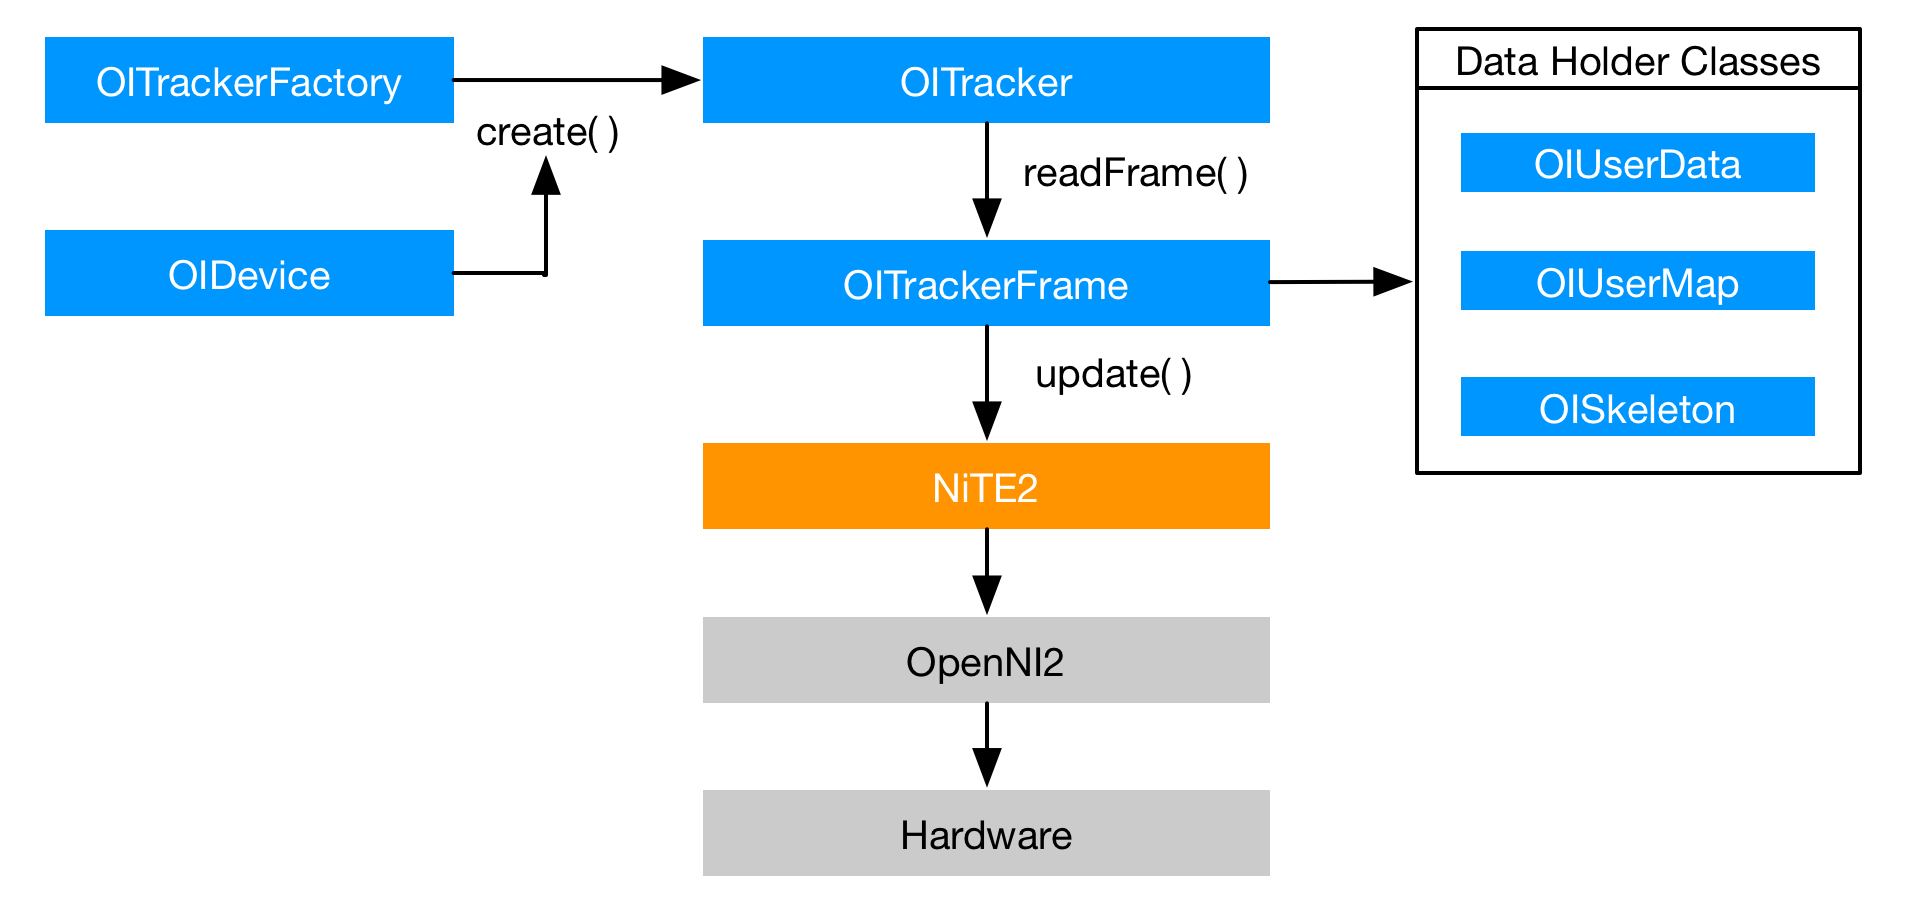
\includegraphics[width=\linewidth]{figures/framework_oitracker_workflow.png}
    \caption[Tracker module interactive diagram]
    {Tracker module interaction diagram,
        the boxes in blue are our framework's components, the box in
        orange is the concrete tracking algorithm implementation, the boxes in
        gray are the low level components.}
    \label{fig:fw-skeleton-workflow}
\end{figure}

In \autoref{sec:fw-inst-tracker}, we showed that the \texttt{OISkeletonTracker}
class implements the \texttt{OIFlowable} interface which means that the
skeleton tracking application will work in the same manner as our ReID
application. With the pipeline mechanism introduced, our first step is to
create a corresponding skeleton tracking pipeline shown as
\autoref{fig:fw-app-skt-pipeline}, then we instantiate the a device filter as
input, a tracker filter to perform tracking and a viewer filter for display.
Next, as what we did for ReID application, we have to create a concrete
\texttt{OIFlowContext} for the skeleton tracking task named
\texttt{OISktFlowContext}.
Finally, we invoke the \texttt{flow} method of the pipeline instance.
The procedure can be described as \autoref{algo:fw-app-skt}.

\begin{figure}
    \centering
    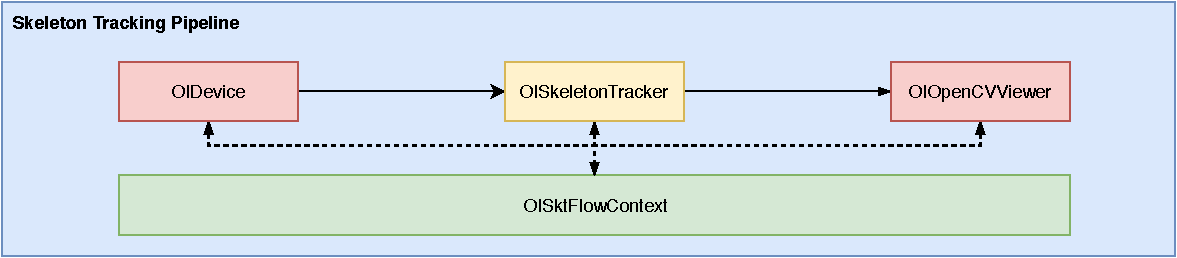
\includegraphics[width=\linewidth]{figures/framework_app_skt_pipeline.pdf}
    \caption[Skeleton tracking application pipeline]
    {Skeleton tracking application pipeline. The solid line arrow represents
    the pipeline execution order and the dash line arrow represents the
    data flow.}
    \label{fig:fw-app-skt-pipeline}
\end{figure}

\begin{algorithm}
    devF $\leftarrow$ create a device factory\;
    tkF $\leftarrow$ create a tracker factory\;
    \;
    noEcsPressed = True\;
    device = devF.create("name of the device")\;
    tracker = tkF.create("name of the tracker")\;
    \;
    sktContext = new OISktFlowContext \;
    sktPL = new OIPipeline(sktContext) \;
    sktPL.push(dev)\;
    sktPL.push(tracker)\;
    sktPL.push(new OIOpenCVViewer)\;
    \;
    \While{noEcsPressed}{
        sktPL.flow(sktContext)\;
        \If{isEcsPressed}{
            noEcsPressed = False\;
        }
    }
    \caption{Skeleton tracking application procedure}
    \label{algo:fw-app-skt}
\end{algorithm}



\section{Other Applications}
\label{sec:Impl-fw-app-other}

Besides the main person re-identification and the skeleton tracking 
application, we have also implemented
some other applications to show the usability of our framework. All the
available samples can be found under the path \texttt{OpenISS/samples/}.
Currently, we have the sample applications shown as \autoref{tab:fw-avail-apps}.
Like most of the popular frameworks did, the samples not only prove our
framework is useful but also serves as the learning material for the 
application developers who want to build software using our framework to learn 
how to use our APIs.
In this section, we will examine some of the applications with their
supported theory behind and the implementation detail.

\begin{table}[]
    \resizebox{\textwidth}{!}{%
    \begin{tabular}{ll}
        \hline
        Sample Name & Description
        \\ \hline
        {\texttt{calib.cpp}}           
        & \begin{tabular}[c]{@{}l@{}}
        	Camera calibration application, which can be used to calibrate 
        	camera\\ by inputting checkerboard images.
        \end{tabular}
        \\ \hline
        {\texttt{kinect\_capture.cpp}}
        & \begin{tabular}[c]{@{}l@{}}
        	Minimum Kinect application, it can stream both color and depth \\ 
        	image of the scene in real time and display on the screen.
        \end{tabular}
        \\ \hline
        {\texttt{kinect\_sklt.cpp}}
        & Skeleton tracking application using Kinect devices.
        \\ \hline
        {\texttt{rs\_capture.cpp}}
        & \begin{tabular}[c]{@{}l@{}}
        	Minimum RealSense application, it can stream both color and \\ 
        	depth image of the scene in real time and display them.
        \end{tabular}
        \\ \hline
        {\texttt{rs\_align.cpp}}
        & \begin{tabular}[c]{@{}l@{}}
        	Image alignment application, it can align the depth image to \\ the 
        	color image captured by RealSense camera and also filter \\ out the 
        	background based on the distance value.
        \end{tabular}
        \\ \hline
        {\texttt{yolo.cpp}}
        & \begin{tabular}[c]{@{}l@{}}
        	Person detection application based on YOLO v3 algorithm \\ 
        	built on top of OpenISS APIs.
        \end{tabular}
        \\ \hline
        {\texttt{reid.cpp}}            
        & Person re-identification application.
        \\ \hline
    \end{tabular}%
    }
    \caption{Available applications provided by OpenISS.}
    \label{tab:fw-avail-apps}
\end{table}

\subsection{Camera Calibration}
\label{sec:Impl-fw-app-calib}

Camera calibration, is one of the basic functionality of a computer 
vision-related library. Because of the limitation of manufacturer craft, the 
intrinsic matrix which is important for a certain camera application among of computer vision 
tasks varies across cameras. 
Also, the pose of camera which is described by the extrinsic matrix is 
another significant parameter as well. 
Camera calibration is a way to obtain both intrinsic and extrinsic matrices as 
well as fixing the distortion issue of the cameras.

\subsubsection{Pinhole Model}

Most of the cameras are using the pinhole model to capture images. 
The pinhole model can be shown as \autoref{fig:fw-pinhole}, where $P(x, 
y, z)$ is a 3D point in the real-world, $P'(x', y')$ is the corresponding point in 
the 2D image plane and $f'$ is the focal length.
What a camera does can be imagined as a mapping relation between the real 
world 3D point and the image's 2D point, illustrated as \autoref{eq:cam}.
If we know the real world poin'st $P$ coordinate, by applying trigonometric 
calculations, we can calculate the coordinate of $P'$ using 
\autoref{eq:pinhold-cartes}.

\begin{equation}
\label{eq:cam}
P=\left[ \begin{array}{l}{x} \\ {y} \\ {z}\end{array}\right] \rightarrow
P^{\prime}=\left[ \begin{array}{l}{x^{\prime}} \\ {y^{\prime}}\end{array}\right]
\end{equation}

\begin{equation}
\label{eq:pinhold-cartes}
\left\{\begin{array}{l}{x^{\prime}=f^{\prime} \frac{x}{z}} \\
{y^{\prime}=f^{\prime} \frac{y}{z}}\end{array}\right.
\end{equation}


\subsubsection{Distortions Removal}

Due to the fact that pinhole cameras may introduce distortion to images, we 
need to understand what is the kind distortion, then figure out how to fix it. There are mainly 
two kinds of distortions, radial and tangential distortion, illustrated by 
\autoref{fig:fw-app-dis}.
According to \cite{paper-camera-calibration}, radial distortion can be solved by
\autoref{eq:radial} and tangential distortion can be solved by
\autoref{eq:tangential}. Then eventually, we need to find five parameters to
describe this model, formulated as \autoref{eq:disortion-model}.

\begin{figure}[ht]
    \centering
    \vbox{\begin{subfigure}
        \centering
        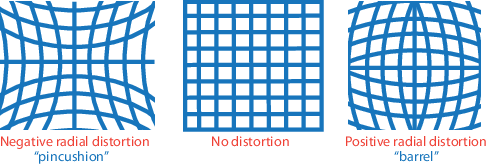
\includegraphics[width=.7\linewidth]{figures/framework_calibration_radial_distortion.png}
        \label{fig:fw-rad-dis}
    \end{subfigure}}
    \vbox{\begin{subfigure}
        \centering
        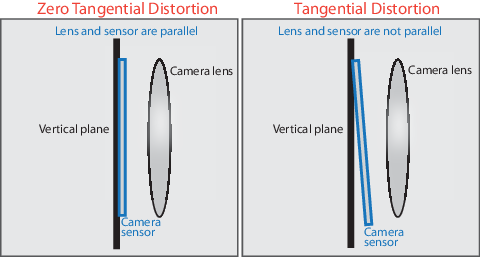
\includegraphics[width=.6\linewidth]{figures/framework_calibration_tangentialdistortion.png}
        \label{fig:fw-tan-dis}
    \end{subfigure}}
    \caption[Two kinds of distortions model]
    {Two kinds of distortion models, the first row represents radial distortion,
        the second row represents tangential distortion 
        \protect\cite{camera-calibration-mathworks}.}
    \label{fig:fw-app-dis}
\end{figure}

\begin{equation}
\begin{aligned} x_{\text {corrected}} &=x\left(1+k_{1} r^{2}+k_{2} r^{4}+k_{3}
r^{6}\right) \\ y_{\text {corrected}} &=y\left(1+k_{1} r^{2}+k_{2} r^{4}+k_{3}
r^{6}\right) \end{aligned}
\label{eq:radial}
\end{equation}

\begin{equation}
\begin{aligned} x_{\text {corrected}} &=x+\left[2 p_{1} x y+p_{2}\left(r^{2}+2
x^{2}\right)\right] \\ y_{\text {corrected}} &=y+\left[p_{1}\left(r^{2}+2
y^{2}\right)+2 p_{2} x y\right] \end{aligned}
\label{eq:tangential}
\end{equation}

\begin{equation}
\text {Distortion coefficients}=\left( \begin{array}{lllll}{k_{1}} & {k_{2}} &
{p_{1}} & {p_{2}} & {k_{3}}\end{array}\right)
\label{eq:disortion-model}
\end{equation}

\subsubsection{Intrinsic and Extrinsic Matrices}
\label{sec:Impl-ins-exs-mat}

Observed from \autoref{eq:pinhold-cartes}, division is not a linear
transformation which is not convenient for calculation. So we move the
coordinate from Cartesian to homogeneous to make the formula linearly
computable, also assuming optical center at $(u_0, v_0)$, pixel shape is
square, no skew exists and no restriction to the camera pose.
Then their relation can be concluded by \autoref{fig:fw-ins-exs-mat} and
formulated by \autoref{eq:ins-exs-mat} where $K$ is the intrinsic matrix, $E$
is the extrinsic matrix, $R$ is the rotation matrix and $\overline{t}$ is the
translation vector.

\begin{figure}
	\centering
    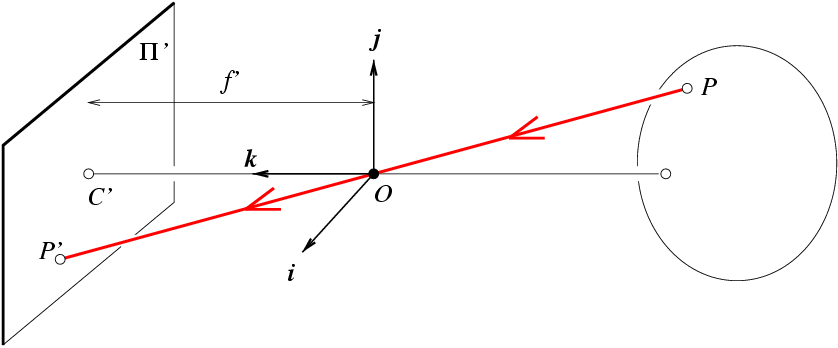
\includegraphics[scale=0.4]{figures/framework_pinhole_camera.png}
    \caption{Pinhole camera model.}
    \label{fig:fw-pinhole}
\end{figure}

\begin{equation}
\label{eq:ins-exs-mat}
P^{\prime} = \left[ \begin{array}{ccc}{f} & {0} & {u_{0}} \\ {0} & {f}
& {v_{0}} \\
{0} & {0} & {1}\end{array}\right] \left[ \begin{array}{llll}{r_{11}} & {r_{12}}
& {r_{13}} & {t_{x}} \\ {r_{21}} & {r_{22}} & {r_{23}} & {t_{y}} \\ {r_{31}} &
{r_{32}} & {r_{33}} & {t_{z}}\end{array}\right] \left[ \begin{array}{l}{x} \\
{y} \\ {z} \\ {1}\end{array}\right]
= K E P = K [R \:\:\: \overline{t}] P
\end{equation}

\begin{figure}
    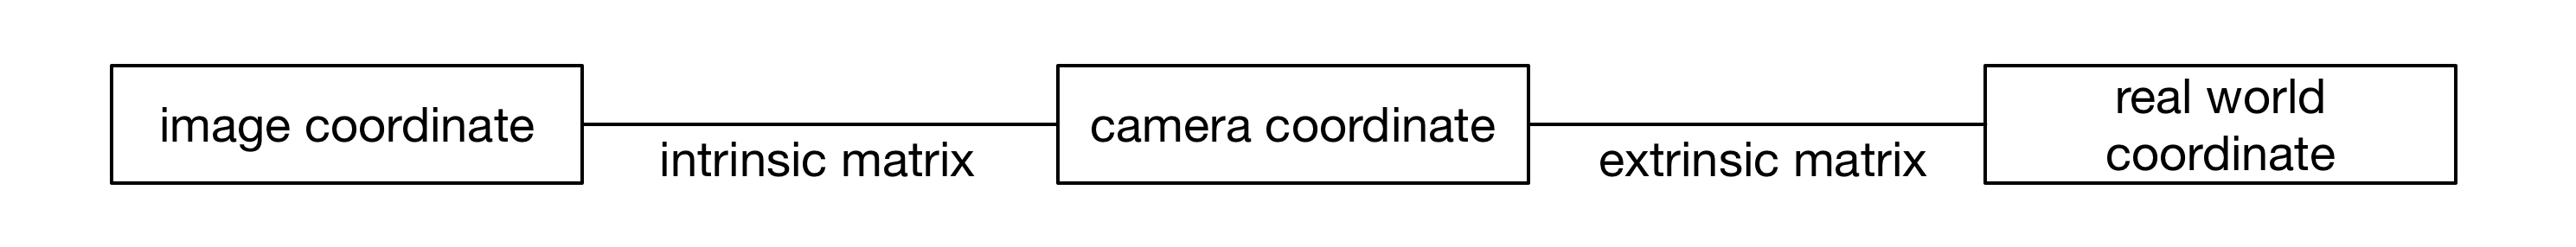
\includegraphics[width=\linewidth]{figures/framework_camera_matrix.png}
    \caption{Relation between three coordinates and camera matrices.}
    \label{fig:fw-ins-exs-mat}
\end{figure}

\subsubsection{Solving Distortion coefficient, Intrinsic and Extrinsic Matrices}

In the camera calibration problem, we need to perform a reverse computation in which
$P$ and $P'$ are known, the unknown being the intrinsic and extrinsic matrices.
So we need to provide some sample images with well-defined pattern 
(typically a checkerboard). Then we detect the corners of the image whose  
positions are known. Finally, we solve the equation system to get our target 
$K$ and $E$ as well as the distortion coefficient.

We already have OpenCV as our dependencies and it has the functionality
that can help us to solve those equations. So what we need to do just input a 
set of images with the pre-defined pattern. 
We break the implementation into several methods, the detailed explanation for 
each of them are listed below. A sample result can be found through 
\autoref{fig:fw-app-calib}.

\begin{enumerate}
    \item \texttt{prepareFileName}, takes a directory that contains all the images
    used for calibration as input, extracts their file path and puts them into a
    vector.
    \item \texttt{prepareObjChessboardCorners}, prepares the pre-defined
    pattern of the corner and stores them into a vector.
    \item \texttt{loadTestingImgAndFindCorner}, invokes OpenCV to load
    the image into memory and uses Haris-Corner detector to find a certain
    amount of corner points within all the loaded images.
    \item \texttt{runCalibration}, takes the pre-defined corners and the
    detected corners as input applying the theory described in the previous 
    section and solve the equation to find the distortion coefficient, 
    intrinsic and extrinsic matrices.
\end{enumerate}

\begin{figure}
    \centering
    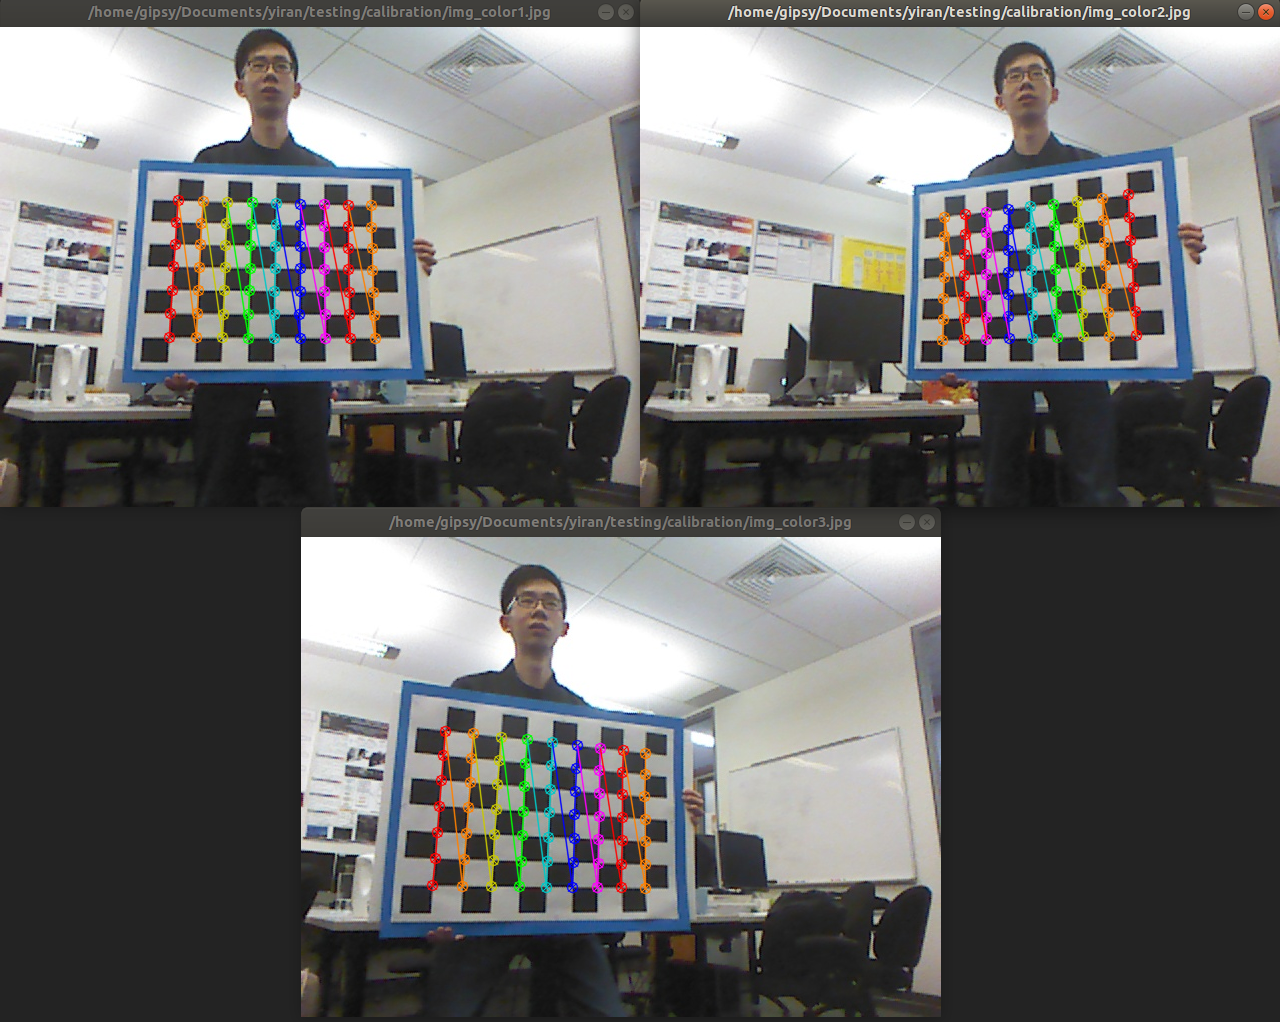
\includegraphics[width=\linewidth]{figures/framework_app_calib.png}
    \caption{Example usage for camera calibration application.}
    \label{fig:fw-app-calib}
\end{figure}

\subsection{Image Alignment}
\label{sec:Impl-fw-app-align}

Since in our solution, we target the depth cameras as the input device, in such
case, we will have not only the normal RGB image but also the depth image (an
image where the value in each pixel is the distance of the object away from the
depth sensor). Take Kinect v2 as an example: from \autoref{fig:fw-kinectv2} we
found that the RGB and depth (IR) sensor are not at the same
position on the camera housing which means that these two images for the same scene cannot be mapped 
pixel to pixel directly. 
An sample image pair before alignment can be shown as 
\autoref{fig:fw-raw-image}. We can see that the person is closer to the image
right-edge in the left image than that in the right image.

\begin{figure}
    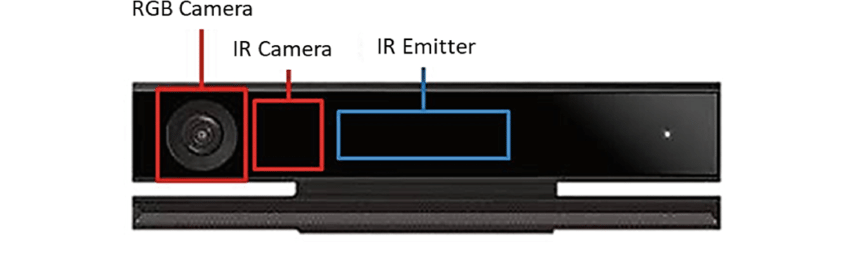
\includegraphics[width=\linewidth]{figures/framework_kinectv2.png}
    \caption{Kinect v2 sensor front with cameras and emitter positions.}
    \label{fig:fw-kinectv2}
\end{figure}

\begin{figure}
    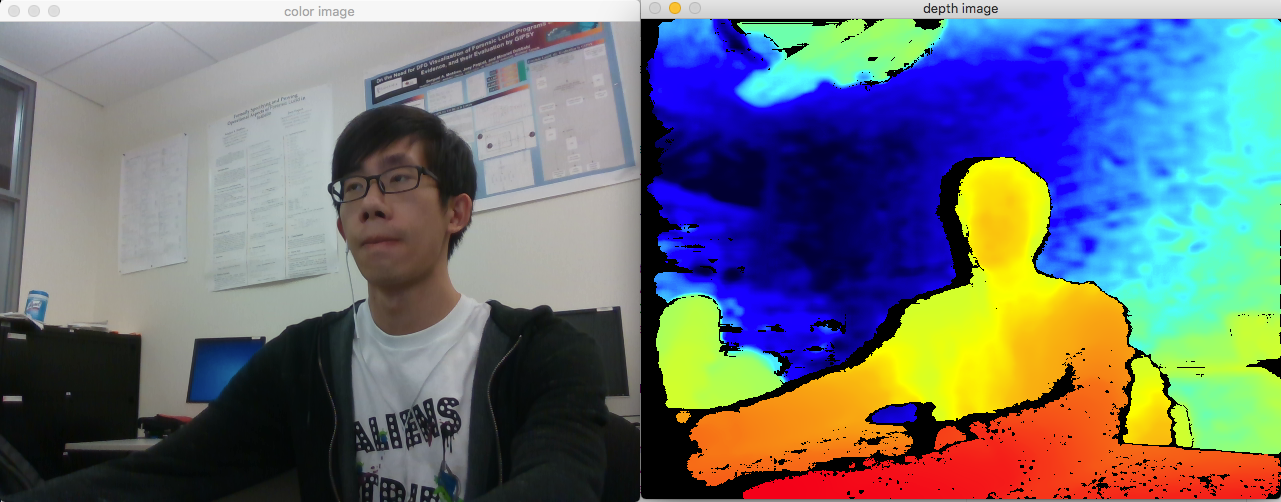
\includegraphics[width=\linewidth]{figures/framework_raw_images.png}
    \caption[Example without alignment]
    {Raw color image and depth image without alignment, we can clearly
        see that there is displacement between these two images.}
    \label{fig:fw-raw-image}
\end{figure}

In this case, what we actually want to do is to align the depth image coordinates to the 
color image coordinates. More precisely, given the two types of image taken
for the same scene at the same time, one is the depth image $I_{depth} = (a, b,
depth)$ and the other is the color image $I_{color} = (m, n, intensity)$. For
each pixel in $I_{depth}$, the alignment problem is to find the corresponding point, where
$realworld(m, n) = realworld(a, b)$, in
$I_{color}$ and expand it to be $(m, n, intensity, depth)$.

Assuming that we already know the matrices of both depth and color cameras denoted by
$K_{intrinsic}^{depth}$, $E_{extrinsic}^{depth}$, $K_{intrinsic}^{color}$ and
$E_{extrinsic}^{color}$, then we loop over all the pixels in the depth image and
try to re-project them onto the color image plane. For each pixel in the depth
image $p_{depth}(x, y)$, we perform the following operations. In our solution, 
this work is done by \texttt{OIAligner} class shown as
\autoref{fig:fw-aligner}.

\begin{enumerate}
    \item With $K_{intrinsic}^{depth}$ and $E_{extrinsic}^{depth}$, we can
    project $p_{depth}(x, y)$ back to the real world coordinate to get
    $P(x', y', z')$.
    \item With $K_{intrinsic}^{color}$ and $E_{extrinsic}^{color}$, we capture
    the re-projected point $P(x', y', z')$ and compute its corresponding
    point $p_{color}(x'', y'')$ in the color image plane.
\end{enumerate}

\begin{figure}
    \centering
    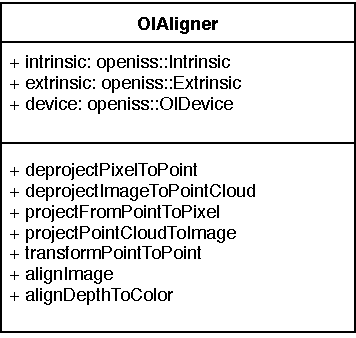
\includegraphics[scale=1.0]{figures/framework_oialigner.pdf}
    \caption{UML class diagram of {\texttt{OIAligner}} class}
    \label{fig:fw-aligner}
\end{figure}

\subsection{Green Screen Image}
\label{sec:Impl-fw-app-green-img}

Green screen image, is a technique which is widely used in the film industry. 
The originally idea is that we shoot a clip in front of a green backdrop then we
apply whatever background we need to replace the green part of the captured image.
In our case, we use this technique for background removal. Basically, it allows us
to remove useless information of the scene depending on the depth value which
maybe useful in some situations. For example, for the person recognition task,
some models may expect the input just to be the person itself without any
other noise, then this functionality becomes extremely helpful.

In our implementation, we provide a GUI for the users to determine
only to keep the information based on a depth value threshold. This function
deeply relies on the two functionalities we mentioned above: camera calibration
and image alignment. Only when the image is aligned, we are able to filter out
the pixel whose deep value is larger than the threshold. An example of the
application can be shown as \autoref{fig:fw-greenscreen}.

\begin{figure}
    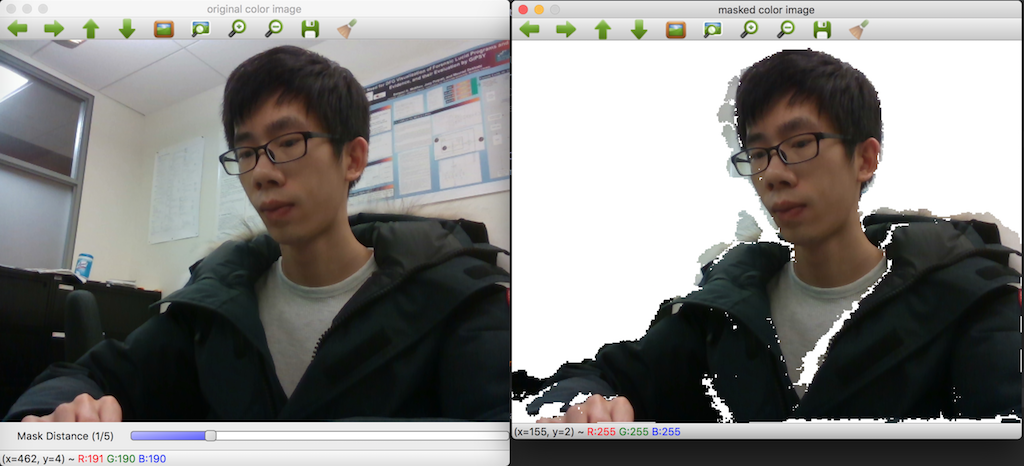
\includegraphics[width=\linewidth]{figures/framework_greenscreen.png}
    \caption[An example of the green screen image]
    {An example of the green screen image, left is the original color
        image and the right is the image after background removal.}
    \label{fig:fw-greenscreen}
\end{figure}

\section{Summary}

In this chapter, we introduced the applications which make use of our framework
instance proposed in \autoref{chap:fw-inst}. In the ReID application, we mainly
focus on the pipeline design architecture provided by our framework, which is the most valuable point of our
framework in this case. With such a mechanism, we can integrate components into the
framework easily, while maintaining a good modular design and these
components can be reused for various tasks.
Then we described three more applications which are common and basic
within computer vision libraries frameworks. 
The camera calibration allows us to obtain more accurate intrinsic and 
extrinsic matrices, the image alignment
enables us to map the depth image to the color image pixel by pixel and the
green screen image makes use of the previous two and provides background
removal functionality that proves useful in various situations.
In the next chapter, we will evaluate our framework solution according to our 
proposed requirements and demonstrate how well our solution can achieve using 
common metrics acknowledged by the community.

% EOF


% ********************************************
% 提纲
%
% 1. ReID 应用
%   - 以前介绍的是 framework,引入 application
%   - 如果是 library 的话,怎么写,引入 pipeline
%   - pipeline 有什么好
%   - pipeline 怎么应用在这里
% 2. Skeleton tracking 应用
% 3. 其他应用
%   - camera calibration
%   - image alignment
%   - green screen image
% ********************************************